%%%%%%%%%%%%%%%%%%%%%%%%%%%%%%%%%%%%%%%%%%%%%%%%%%%%%%%%%%%%%%%%%%%%%%%%%%%%%%%%
%2345678901234567890123456789012345678901234567890123456789012345678901234567890
%        1         2         3         4         5         6         7         8

%\documentclass[journal,transmag]{IEEEtran}% Comment this line out if you need a4paper

\documentclass[10pt, conference]{ieeeconf}      % Use this line for a4 paper

\IEEEoverridecommandlockouts                              % This command is only needed if 
                                                          % you want to use the \thanks command

%\overrideIEEEmargins                                      % Needed to meet printer requirements.

% See the \addtolength command later in the file to balance the column lengths
% on the last page of the document

% The following packages can be found on http:\\www.ctan.org
%\usepackage{graphics} % for pdf, bitmapped graphics files
%\usepackage{epsfig} % for postscript graphics files
%\usepackage{mathptmx} % assumes new font selection scheme installed
%\usepackage{times} % assumes new font selection scheme installed
%\usepackage{amsmath} % assumes amsmath package installed
%\usepackage{amssymb}  % assumes amsmath package installed

\newtheorem{theorem}{Theorem}[section]
\newtheorem{lemma}[theorem]{Lemma}
\newtheorem{proposition}[theorem]{Proposition}
\newtheorem{corollary}[theorem]{Corollary}
\usepackage[ruled,vlined]{algorithm2e}

\newcommand{\qed}{\nobreak \ifvmode \relax \else
      \ifdim\lastskip<1.5em \hskip-\lastskip
      \hskip1.5em plus0em minus0.5em \fi \nobreak
      \vrule height0.75em width0.5em depth0.25em\fi}

\def\lc{\left\lfloor}   
\def\rc{\right\rfloor}

\usepackage{amsmath,amssymb}

\usepackage{tabularx}
\usepackage{tikz,hyperref,graphicx,units}
\usepackage{subfigure}
\usepackage{benktools}
\usepackage{bbm}
\renewcommand{\baselinestretch}{.5}

\usepackage{caption}
\usepackage{epstopdf}
\renewcommand{\captionfont}{\footnotesize}
\usepackage{sidecap,wrapfig}
\usepackage[ruled,vlined]{algorithm2e}
\DeclareMathOperator*{\argmin}{arg\,min}
\DeclareMathOperator*{\argmax}{arg\,max}
\newcommand{\abs}[1]{\lvert#1\rvert} 
\newcommand{\norm}[1]{\lVert#1\rVert}
%\newcommand{\suchthat}{\mid}
\newcommand{\suchthat}{\ \big|\ }
\newcommand{\ba}{\mathbf{a}}
\newcommand{\bb}{\mathbf{b}}
\newcommand{\bc}{\mathbf{c}}
\newcommand{\bd}{\mathbf{d}}
\newcommand{\bg}{\mathbf{g}}
\newcommand{\bj}{\mathbf{j}}
\newcommand{\bn}{\mathbf{n}}
\newcommand{\bp}{\mathbf{p}}
\newcommand{\bw}{\mathbf{w}}
\newcommand{\bt}{\mathbf{t}}
\newcommand{\bu}{\mathbf{u}}
\newcommand{\by}{\mathbf{y}}
\newcommand{\bx}{\mathbf{x}}
\newcommand{\bz}{\mathbf{z}}
\newcommand{\bbf}{\mathbf{f}}
\newcommand{\bzero}{\mathbf{0}}
\newcommand{\bG}{\mathbf{G}}
\newcommand{\bA}{\mathbf{A}}
\newcommand{\bW}{\mathbf{W}}
\newcommand{\bX}{\mathbf{X}}
\newcommand{\mX}{\mathcal{X}}
\newcommand{\mD}{\mathcal{D}}
\newcommand{\mG}{\mathcal{G}}
\newcommand{\mN}{\mathcal{N}}
\newcommand{\mW}{\mathcal{W}}
\newcommand{\mF}{\mathcal{F}}
\newcommand{\bZ}{\mathbf{Z}}
\newcommand{\mR}{\mathcal{R}}

\newcommand{\bfc}{W}
\newcommand{\Qinf}{Q_{\infty}}
\newcommand{\st}[1]{_\text{#1}}
\newcommand{\rres}{r\st{res}}
\newcommand{\pos}[1]{(#1)^+}
\newcommand{\depth}{\operatorname{depth}}
\newcommand{\dist}{\operatorname{dist}}
\newcommand{\convhull}{\operatorname{ConvexHull}}
\newcommand{\minksum}{\operatorname{MinkowskiSum}}

\newcommand{\specialcell}[2][c]{ \begin{tabular}[#1]{@{}c@{}}#2\end{tabular}}
\newcommand{\acro}{SHIV}
\newcommand\independent{\protect\mathpalette{\protect\independenT}{\perp}}
\def\independenT#1#2{\mathrel{\rlap{$#1#2$}\mkern2mu{#1#2}}}

\newcolumntype{L}[1]{>{\RaggedRight\hspace{0pt}}p{#1}}
\newcolumntype{R}[1]{>{\RaggedLeft\hspace{0pt}}p{#1}}


\newboolean{include-notes}
\setboolean{include-notes}{false}
\newcommand{\adnote}[1]{\ifthenelse{ \boolean{include-notes}}%
 {\textcolor{blue}{\textbf{AD: #1}}}{}}
 
 \newcommand{\fpnote}[1]{\ifthenelse{ \boolean{include-notes}}%
 {\textcolor{blue}{\textbf{FP: #1}}}{}}
 
  \newcommand{\mlnote}[1]{\ifthenelse{ \boolean{include-notes}}%
 {\textcolor{purple}{\textbf{ML: #1}}}{}}

\renewcommand{\baselinestretch}{.92}


%\title{Iterative Imitation Learning with Reduced Human Supervision [v11]}
%\title{SHIV:  Reducing Human Supervision for Robot Active Learning [v11]}

\title{SHIV: Reducing Supervisor Burden using Support Vectors for Efficient
Learning from Demonstrations in High Dimensional State Spaces }



\author{Michael Laskey$^1$, Sam Staszak$^1$, Wesley Yu-Shu Hsieh$^1$, Jeffrey Mahler$^1$, \\ Florian T. Pokorny$^1$, Anca D. Dragan$^1$, and Ken Goldberg$^{1,2}$% <-this % stops a space
\thanks{$^1$ Department of Electrical Engineering and Computer Sciences; {\small \{mdlaskey,iamwesleyhsieh,ftpokorny,anca\}@berkeley.edu, \small staszass@rose-hulman.edu} }%
\thanks{$^2$ Department of Industrial Engineering and Operations Research; {\small goldberg@berkeley.edu}}%
\thanks{$^{1-2}$ University of California, Berkeley;  Berkeley, CA 94720, USA}%
}
\begin{document}



\maketitle
\thispagestyle{empty}
\pagestyle{empty}


%%%%%%%%%%%%%%%%%%%%%%%%%%%%%%%%%%%%%%%%%%%%%%%%%%%%%%%%%%%%%%%%%%%%%%%%%%%%%%%%

\begin{abstract}
Online learning from demonstration algorithms, such as DAgger, can learn policies for problems where the system
dynamics and the cost function are unknown. However, during learning, they impose a burden on supervisors to provide labels (control
signals) as the robot encounters new states while executing its current best policy. We introduce the SHIV
algorithm (Svm-based reduction in Human InterVention), which reduces this burden by only requesting supervision for risky states. SHIV uses stream-based active learning with a query selection method that evaluates risk in a manner tailored to non-stationary high dimensional state distributions.  To facilitate scaling and outlier rejection, risk is based on distance to an approximate level set boundary defined by a One Class support vector machine.  We compare SHIV with DAgger in three policy learning experiments: 1) a driving simulator with a 27936 dimension visual HOG feature state representation, 2) a push-grasping in clutter simulation for a 4DOF robot arm, using Box2D, with a 22 dimension state representation  of joint angles and the pose of each object, and 3) a surgical needle insertion task with a 16 dimension state represented spatial transform.  Results suggest that SHIV can learn equivalent policies with up to 70\% fewer queries.

 \end{abstract}


%%%%%%%%%%%%%%%%%%%%%%%%%%%%%%%%%%%%%%%%%%%%%%%%%%%%%%%%%%%%%%%%%%%%%%%%%%%%%%%%

\section{Introduction} 


In model-free robot Learning from Demonstration (LfD), a robot learns to perform a task, such as driving or grasping an object in a cluttered environment, from examples provided by a  supervisor, usually a human.  In such problems, the robot does not have access to either the cost function that it should optimize, nor the dynamics model. The former occurs when it is difficult to specify how to trade-off various aspects that matter, like a car trying to drive on the road and dodge other cars \cite{abbeel2004apprenticeship}.  The latter occurs when either the system or the interaction with the world is difficult to characterize, like when a robot is trying to grasp an object in clutter and does not have an accurate model of the objects dynamics. 

Rather than explicitly learning the cost function (like in Inverse Reinforcement Learning \cite{ng2000algorithms}) and the dynamics model, and then using optimization to produce a policy for the task, in model-free LfD the robot learns the policy directly from supervisor examples, mapping states to controls~\cite{argall2009survey}. Learning from demonstration has been used successfully in recent year for a large number of robotic tasks, including helicopter maneuvering \cite{abbeel2007application},car parking \cite{abbeel2008apprenticeship},  and robotic surgery \cite{van2010superhuman}. 

 


\begin{figure}[ht]
\centering
   
\includegraphics[width=0.5\textwidth]{figures/teaser.pdf}
\caption{ \footnotesize
SHIV  reduces the number of queries to the supervisor in our three test domains: a) a driving simulator where the goal is to learn a controller on HOG features extracted from synthetic images to keep a car on a polygonal track; b) push-grasping in clutter in a physics simulator, where the goal is to learn a controller from human demonstrations to grasp the green object while not letting the red square objects fall off the gray boundary representing a table; c) learning a controller for the Da Vinci Research Kit from a master surgeon's demonstrations of correcting a needle before suturing in surgery; d) normalized performance of SHIV and DAgger's policy on the grasping in clutter example versus states labeled by the supervisor.
}
\vspace*{-20pt}
\label{fig:teaser}
\end{figure}




LfD algorithms can be categorized as offline, where the robot only observes demonstrations, or online, where the robot interacts with the world and receives feedback from the supervisor.
In offline LfD, the robot learns the policy based on a batch of examples, and then executes it to achieve the task.  During execution, a small error can accumulate, leading the robot away from the region of the state space where it was given examples, leading to unrecoverable failures.  For example, a robot driving may be trained on examples driving safely down the center of a lane, but even slight deviations will eventually put the robot into states near the side of the road where its policy could  fail~\cite{pomerleau1989alvinn}. Ross and Bagnell showed the number of errors made by the robot, in the worst case,  can scale quadratically with the time horizon of the task~\cite{ross2010efficient}.




Online LfD addresses this issue by iteratively gathering more examples from the supervisor in states the robot encounters~\cite{grollman2007dogged,ross2010efficient,ross2010reduction}. One such algorithm, DAgger, learns a series of policies. At each iteration, the robot trains a policy based on the existing examples, then rolls out (executes) that policy, and the supervisor provides demonstrations for all states the robot visits. The new state/control examples are aggregated with the old examples for the next iteration. DAgger and related algorithms have been applied in a wide range of applications, from quadrotor flight to natural language to Atari games~\cite{NIPS2014_5421,duvallet2013imitation,ross2013learning}. In DAgger, under certain conditions, the number of errors scales only linearly with the time horizon of the task\cite{ross2010reduction}.

However one drawback is that DAgger significantly increases the burden on the supervisor, who now labels all states that the robot visits during training.  Our goal is to reduce supervisor burden without degrading performance.

Our key insight is that the robot only needs to request demonstrations for risky states. Risk arises because:  (1) states are sufficiently different than the states previously encountered, i.e., they can be considered novel or outliers~\cite{hodge2004survey}; or (2) states are in a region that has been misclassified in previous training data.
%\adnote{Ken's version below does not seem to represent what we actually do.}
%the action associated with a state under the current policy yield a resulting state that is inconsistent with the expected next state. [how do we measure 2? - Ken]


We present an algorithm for online LfD that can actively decide whether it is necessary to ask the supervisor to label the new states that the robot encounters. SHIV  (Svm-based reduction in Human InterVention) reduces supervisor burden by only requesting supervision for risky states. SHIV uses stream-based active learning with a query selection method that evaluates risk in a manner tailored to the non-stationary state distributions the robot encounters as it iteratively executes learned policies, and tailored to high dimensional state spaces. We build on the One Class SVM method for approximating quantile level sets \cite{scholkopf2001estimating} to provide a classification method for deciding if a state is risky or safe.


\adnote{nothing about experiements and resutls? how do i know if it worked? also how do i know that you didn;t just compare to dagger, but ran an indepth analysis of the algorithm? i thought i put a paragraph like that here at some point}



\section{Related Work}
Below we summarize related work in active approaches to robot LfD and risk evaluation techniques.

\noindent\textbf{Active Learning from Demonstration}
We formulate reducing supervisor burden in nnline Lfd as a stream-based active learning problem ~\cite{atlas1990training,cohn1994improving}. In stream based active learning, the decision of whether to query the supervisor (for a label or control signal) or not is not over the entire state space (like in traditional pool-based active learning), but on states drawn one at a time from some data stream. In  online LfD, this data stream is the states encountered when the robot is executing the current best policy.

Aside from the data stream, stream-based active learning has another ingredient: a query selection method, deciding whether or not to query. Typical query selection methods are estimator-centric, evaluating risk using the estimator, e.g. distance from the classification hyperplane \cite{tong2002support}, as in Fig. \ref{fig:support_example}(a); or query by committee  \cite{breiman1996bagging}, which uses a committee of hypothesized estimators that are trained on different subsets of the training data. Risk in query by committee is based on the level of agreement or disagreement among these hypotheses, with higher levels of disagreement for a state leading to higher chances of querying that state (Fig. \ref{fig:support_example}(b)).

Both approaches implicitly assume a stationary state distribution --- that the new data is sampled from the same distribution as the previous training data. Although such methods have been previously proposed for online LfD (see \cite{chernova2009interactive,grollman2007dogged} for the former and \cite{judah2011active,judah2012active} for the latter),
online LfD violates the stationary distribution assumption because each new policy induces a new distribution of states. This can have negative consequences for learning: it has been shown that when training and test distributions are different, query by committee can perform worse than randomly selecting  which states to query \cite{burbidge2007active}.

The problem lies in being estimator-centric. The  estimator is a function of the current distribution. Therefore, it no longer provides a good measure of confidence when that distribution changes. And the distribution does change when the robot is rolling out a learned policy and starts encountering further away states. Instead of relying on the estimator, our measure of risk explicitly identifies when states are drawn from a different distribution, i.e. when they are novel. Our experiments in Section \ref{sec:experiments} suggest that our measure of risk is more accurate in online LfD problems than estimator-centric measures.

%%In SHIV, we use a query selection method that allows for a non-stationary distribution, evaluating risk based on novelty (is the state an outlier to the training distribution), as in Fig. \ref{fig:support_example}(c). Additionally, we also assign higher risk to  historically mislabeled regions, as in Fig. \ref{fig:support_example}(d). We then use a classification method based on the One Class SVM \cite{scholkopf2001estimating} to predict if a state is risky or not risky, which we we define as safe.%Our approach builds on the One Class SVM method for approximating quantile level sets \cite{}, which has already been used in novelty detection on high-dimensional image data \cite{}. 


\noindent\textbf{Risk via Novelty Detection}
The main motivation for our risk definition is the notion that a trained model will be able to generalize within the distribution it is
trained on \cite{tokdar2010importance}, making states outside of this distribution risky. Novelty detection \cite{hodge2004survey} is concerned with recognizing when this happens: recognizing that a sample is outside of this distribution.

Our work builds on Kim et al. \cite{kim2013maximum} who apply novelty detection to safe online LfD to enable a supervisor to take over and prevent unsafe states.  In their MMD-LI algorithm, risk is evaluated with Maximal Mean Discrepancy. For a single state, this is the sum of a kernel density estimate and the variance of the dataset, which works well in low dimensional state spaces.  MMD-LI also reduces supervisor burden because the supervisor only takes over in risky states, as opposed to providing labels for all new states. 
In contrast, we focus on active learning for online LfD in high-dimensional state spaces. Unlike safe learning, our problem does not require the supervisor to take over. This enables us to avoid the supervisor biasing the states sampled (which can in practice lead to a loss in performance \cite{ross2010reduction}), and also avoid assuming the supervisor is always available. On the other hand, our problem does require novelty detection in high dimensional state spaces, where non-parametric density estimation does not scale very well: it can require data exponential in the dimension of the state space \cite{nadaraya1964estimating}. Our results (Section \ref{sec:experiments}) suggests that in our high dimensional state spaces, SHIV achieves an error rate half of that of kernel density estimate-bases techniques like MMD.
%However, having the supervisor take over can bias the states sampled, which can in practice lead to a loss in performance \cite{ross2010reduction}. In contrast, we focus on active learning for online LfD for high-dimensional state spaces, do not assume the supervisor is always available, and propose an alternative to non-parametric density estimation which can require data exponential in the dimension of the state-space \cite{nadaraya1964estimating}.

An alternative to kernel density estimates is to measure distance to its nearest neighbors \cite{knox1998algorithms}. However, this approach was shown to be
susceptible to issues, since nearest neighbors  incorporates only local information about the data. For example, a group of outliers can be close together, but significantly far from the majority of the data and nearest neighbors would mark them as not novel \cite{hodge2004survey}.

Our approach is based on the One Class SVM proposed by Scholk{\"o}pf et al., which estimates a particular quantile level set for the training data by solving a convex quadratic program  to the find support
vectors~\cite{scholkopf2001estimating}. The method has been theoretically shown to approximate the quantile levelset of a density estimate
asymptotically for correctly chosen bandwidth settings and in the case of a normalized Gaussian kernel function \cite{vert2006consistency}. 
In \cite{liu2014unsupervised}, the One Class SVM has furthermore been used for novelty detection in high-dimensional image data. To our knowledge, incorporating a query selection method for high-dimensional spaces and nonstationary distributions, such as the One Class SVM, into online LfD is a novel contribution.




\section{Problem Statement}
The goal of this work is to learn a policy that matches that of the supervisor's while asking the supervisor for as few examples as possible.


\noindent\textbf{Modeling Choices and Assumptions}  We model the system dynamics as Markovian, stochastic, and stationary. Stationary dynamics occur when, given a state and a control, the probability of the next state does not change over time. Note this is different from the non-stationary distribution over the states the robot encounters during learning. 

We model the initial state as sampled from a distribution over the state space.
We assume a known state space and set of controls. We also assume access to a robot or simulator, such that we  can sample from the state sequences induced by a sequence of controls.   Lastly, we assume access to a supervisor who can, given a state, provide a control signal label. We additionally assume the supervisor can be noisy and imperfect, noting that the robot cannot surpass the level of performance of the supervisor. 

\noindent\textbf{Policies and State Densities.}
Following conventions from control theory, we denote by $\mathcal{X}$ the set consisting of observable states for a robot task, consisting, for example, of 
high-dimensional vectors corresponding to images from a camera, or robot joint angles and object poses in the environment.
We furthermore consider a set $\mathcal{U}$ of allowable control inputs for the robot, which can be discrete or
continuous. We model dynamics as Markovian, such that the probability of state $\mathbf{x_{t+1}}\in
\mathcal{X}$ can be determined from the previous state $\mathbf{x}_t\in\mathcal{X}$ and control input $\mathbf{u}_t\in
\mathcal{U}$: 
$$p(\bx_{t+1}|\bu_{t},\bx_{t}, \ldots, \bu_{0}, \bx_{0})=p(\bx_{t+1}|\bu_{t}, \bx_t)$$
We assume a probability density over initial states $p(\bx_0)$.
%We denote the probability density over the initial state also by $p:\mathcal{X}\to \mathbb{R}$. 

A trajectory $\hat{\tau}$ is a finite series of $T+1$ pairs of states visited and corresponding
control inputs at these states, $\hat{\tau} = (\mathbf{x}_0,\mathbf{u}_0, ...., \mathbf{x}_T,\mathbf{u}_T)$, where $\bx_t\in \mathcal{X}$
and $\bu_t\in \mathcal{U}$ for $t\in \{0, \ldots, T\}$ and some $T\in \mathbb{N}$.  
For a given trajectory $\hat{\tau}$ as above, we denote by ${\tau}$ the corresponding trajectory in state space,
${\tau} = (\bx_0,....,\bx_T)$.


A policy is a function $\pi: \mathcal{X} \to \mathcal{U}$ from states to control inputs. 
We consider a space of policies $\pi_{\theta}:\mathcal{X}\to \mathcal{U}$ parameterized by some $\theta\in \mathbb{R}^d$. Any such policy $\pi_{\theta}$ in an environment with probabilistic initial state density and Markovian dynamics
induces a density on trajectories of length $T+1$: $$p(\tau | \theta)=
p(\bx_0)\prod_{i=0}^{T-1}p(\bx_{t+1}|\pi_{\theta}(\bx_t),\bx_t)$$


Let $p(\bx_t|\theta)$ denote the value of the density of states visited at time $t$ if the robot follows the policy
$\pi_{\theta}$ from time $0$ to time $t-1$.  Following \cite{ross2010reduction}, we can compute
the average density on states for any timepoint by $p(\bx|\theta) = \frac{1}{T} \sum^T_{t=1} p(\bx_t|\theta)$.


While we do not assume knowledge of the distributions corresponding to: $p(\bx_{t+1}|\bx_t,\bu_t)$, $p(\bx_0)$, $p(\bx_t|
\theta)$ or $p(\bx|\theta)$, we assume that we have a stochastic real robot or a simulator such that for any state
$\bx_t$ and control $\bu_t$, we can sample the $\bx_{t+1}$ from the density $p(\bx_{t+1}|\pi_{\theta}(\bx_t),\bx_t)$. 
Therefore, when 'rolling out' trajectories under a policy
$\pi_{\theta}$, we utilize the robot or a simulator to sample the resulting stochastic trajectories rather than
estimating $p(\bx|\theta)$ itself.

\noindent\textbf{Objective.} The objective of  policy learning is to find a policy that minimizes some known cost function $C(\hat{\tau}) = \sum^T_{t=1} c(\bx_t,\bu_t)$ of a trajectory $\hat{\tau}$. The cost $c:\mathcal{X}\times \mathcal{U}\to \mathbb{R}$ is typically user defined and task specific. 
For example, in the task of inserting a peg into a hole, a function on distance between the peg's current and desired final state is used \cite{levine2015end}.  

In our problem, we do not have access to the cost function itself. Instead, we only have access to 
a supervisor that can achieve a desired level of performance on the task. The supervisor provides the robot an initial set
an initial set of $N$ stochastic demonstration trajectories $\lbrace \tilde{\tau}^1,...,\tilde{\tau}^N \rbrace$. 
which are the result of the supervisor applying this policy. This induces a training data set $\mathcal{D}$ of all state-control input pairs from the demonstrated trajectories. 

We define a `surrogate' loss function as in \cite{ross2010reduction}, $l:\mathcal{U}\times \mathcal{U}\to \mathbb{R}$, which provides a distance
measure between any pair of control values. In the continuous case, we consider $l(\bu_0,\bu_1) = ||\bu_0-\bu_1||^2_2$,
while in the discrete case $l(\bu_0,\bu_1) = 1$ if $\bu_0 \neq \bu_1$ and $l(\bu_0, \bu_1)=0$ otherwise.

Given a candidate policy $\pi_{\theta}$, we then use the surrogate loss function to approximately measure how `close' the policy's
returned control input $\pi_{\theta}(\bx)\in \mathcal{U}$ at a given state $\bx\in \mathcal{X}$ is to the supervisor's policy's control output
$\tilde{\pi}(\bx)\in \mathcal{U}$. The goal is to produce a policy that minimizes the surrogate loss relative to the supervisor's policy.


Following \cite{ross2010reduction}, our objective is to find a policy $\pi_{\theta}$ minimizing the expected surrogate loss, where the expectation is taken over the distribution of states induced by the policy across any time point in the horizon:

 \vspace{-2ex}
\begin{align}\label{eq:LFD_obj}
\underset{\theta}{\min} \: E_{p(\bx|\theta)} [l(\pi_\theta(\bx),\tilde{\pi}(\bx))]
\end{align}

 If the robot could learn the policy  perfectly, this state density would match the one encountered in user examples. But if the robot makes an error, that error changes the distribution of states that the robot will visit, which can lead to states that are far away from any examples and difficult to generalize to ~\cite{pomerleau1989alvinn}.This motivates iterative algorithms like DAgger, which iterate between learning a policy and the supervisor providing feedback. The feedback is in the form of control signals on states sampled from the robot's new distribution of states. 

\section{Risky and Safe States}

\begin{figure*}[t]
\centering

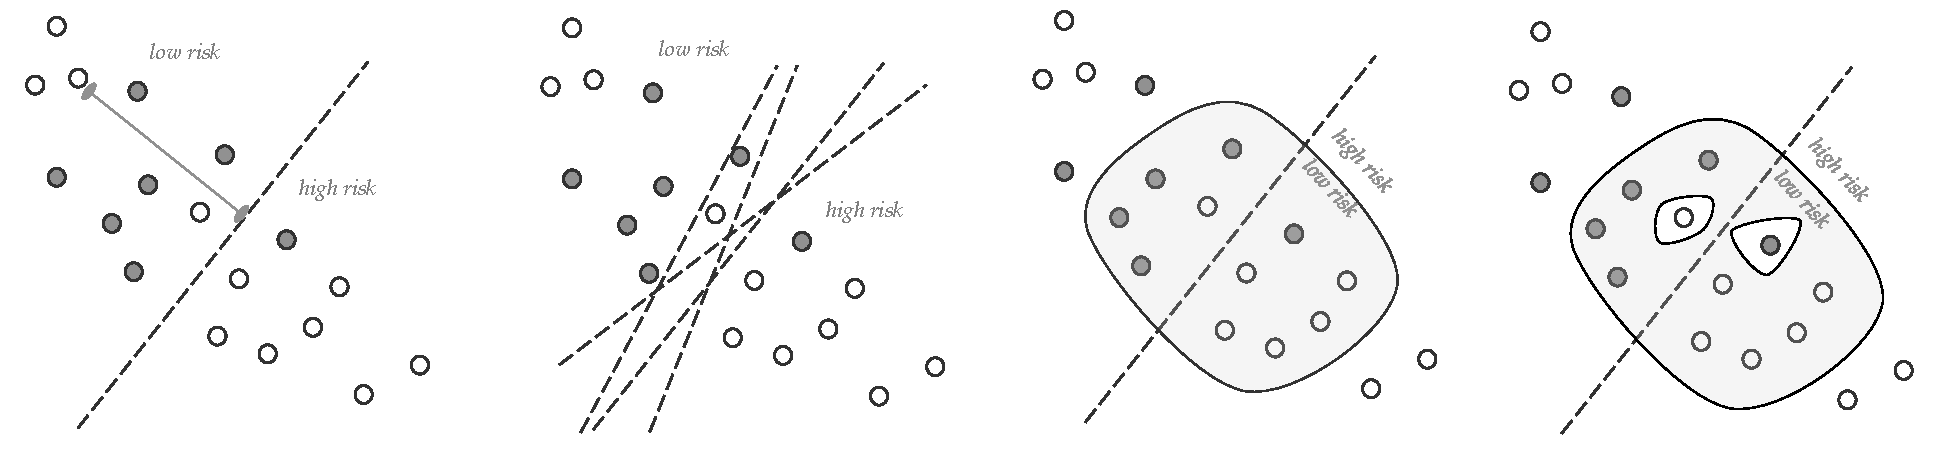
\includegraphics[width=\textwidth]{figures/active_learning.pdf}

\caption{\footnotesize A comparison of different query selection strategies for active learning on a non-stationary distribution. The shaded and empty circles are training data from two classes, $1$ and $0$ respectively. The red empty circles are samples from a new distribution (produced by executing the learned policy), and belong to class $0$. Typical strategies classify states close the decision boundary as risky(a), or for which a set of estimators disagree (b). Neither of these apply to our new samples in red. In contrast, we use a strategy that is amenable to non-stationary distributions by classifying  novel states as safe (i.e not risky) (c) and states in historically mislabeled regions. }
\vspace*{-20pt}
\label{fig:support_example}
\end{figure*}



Providing correct control inputs for (or ``labeling'')  all states encountered at each
iteration can impose a large burden on the supervisor.
Instead of asking the supervisor for labels at all visited states, SHIV uses a measure of risk to actively decide whether a label is necessary. 

In contrast to the standard measure risk based purely on variance, we define a state as "risky" for 2 reasons: 1) it lies in an area with a low density of
previously trained states, which can cause the current policy to mis-predict the supervisor and incur high surrogate
loss~\cite{tokdar2010importance}, or 2) the surrogate loss, or training error, of the current policy at the state  is high, so that the state is unlikely to model the supervisor's control inputs correctly. States that are not classified as "risky" are deemed "safe" .Our definition of risk can be visualized in Fig. \ref{fig:support_example}(d).  

The amount of data needed to estimate the density, scales exponentially in the dimension of the state space~\cite{nadaraya1964estimating}. 
Thus, to evaluate risk in high-dimensional state spaces, such as the HOG features in our driving simulator, Fig. \ref{fig:teaser}(a), we use
a modified version of the technique known as the One Class SVM that  estimates a regularized boundary of a user defined quantile on the training data in $\mathcal{X}$~\cite{scholkopf2001estimating}.
%\fpnote{Refer to figure, replace "one way to do"  by "an approach to this problem is to" or similar - less informal}



%\subsection{Estimation of Quantile Level Sets}\label{sec:level}
We consider the problem of estimating the quantile level-sets of a distribution $P$ on a set $\mathcal{X}$ by means of a finite set of
independent and identically distributed samples $\mathbf{x}_1,...,\mathbf{x}_n\in \mathcal{X}$.
In most general terms, the quantile function for $P$ and subject to a class of measurable subsets $\mathcal{G}$ of $\mathcal{X}$ is
defined by
\vspace{-2ex}
\begin{align}\label{eq:quantile}
U(\gamma) = \mbox{inf} \lbrace \lambda(G):P(G) \geq \gamma, G \in \mathcal{G} \rbrace \: 0<\gamma \leq 1
\end{align} 
$\lambda:\mathcal{G}\to \mathbb{R}$ above denotes a volume measure.
Suppose furthermore that $G:[0,1]\to \mathcal{G}$ assigns a set $G(\gamma) \in \mathcal{G}$ that attains the infinum
measure (i.e. volume) for each $\gamma\in [0,1]$ (this set is in general not necessarily unique). 
$G(\gamma)$ denotes a set of minimum measure $G \in \mathcal{G}$ with $P(G(\gamma))\ge \gamma$. Note in particular that $G(1)$ is the support of the density $p$ corresponding to $P$, if $p$ exists. 

To handle distributions defined on high-dimensional spaces $\mathcal{X}$, work by Scholk{\"o}pf et al. represents the class $\mathcal{G}$ via a kernel $k$ as the set of half-spaces in the support vector (SV) feature space \cite{scholkopf2001estimating}. 
By minimizing a support vector regularizer controlling the smoothness of the estimated level set function this work
derives an approximation of the quantile function described in Eq. \ref{eq:quantile}.
This approach can be thought of as employing $\lambda(G) = ||w||^2$, where $G_w = \lbrace x: f_w(x) \geq \rho \rbrace$,
$f_w(\mathbf{x}) = \sum_i w_i k(\mathbf{x}_i, \mathbf{x})$
and $(w,\rho)$ denote the weight vector and offset parameterizing a hyperplane in the feature space associated with a
Gaussian kernel $k(\bx_0,\bx_1) = e^{-||\bx_0 - \bx_1||^2/2\sigma^2}$.


Let $\Phi:\mathcal{X}\to \mathcal{F}$ denote the feature map corresponding to our exponential kernel, mapping the
observation space $\mathcal{X}$ into a Hilbert space $(\mathcal{F}, \langle, \rangle)$ such that $k(\bx, \bx') = \langle
\Phi(\bx), \Phi(\bx')\rangle$.

The One Class SVM proposed by \cite{scholkopf2001estimating} determines a hyperplane in feature space $\mathcal{F}$
maximally separating the input data from the origin:
\vspace{-2ex}
\begin{align}\label{eq:primal_sup}
    \underset{w\in \mathcal{F}, \mathbf{\xi} \in \mathbb{R}, \rho \in \mathbb{R}}{\mbox{minimize}}\: \frac{1}{2}||w||^2+\frac{1}{vn} \sum^n_i \xi_i - \rho\\
\mbox{s.t} \: \langle w,\Phi(x_i) \rangle \geq \rho - \xi_i, \: \xi_i \geq 0 \notag.
\end{align}

Here, the parameter $\nu$ controls the penalty or `slack term' and is equivalent to $\gamma$ \cite{vert2006consistency}
in the quantile definition, Eq. \ref{eq:quantile}, as the number of samples increases. The decision
function, determining point membership in the approximate quantile levelset is given by $g(\bx) = \mbox{sgn}(\langle w,\Phi(x) \rangle-\rho)$. Here, for $x\in \mathcal{X}$, $g(x)=0$ if $x$ lies on the quantile levelset,
$g(x) = 1$ if $x$ is strictly in the interior of the quantile super-levelset and $g(x) = -1$ 
if $x$ lies strictly in the quantile sub-levelset. 



The dual form of the optimization yields a Quadratic Program 
that has worst case computational complexity of $O(n^3)$. However, Sch{\"o}lkopf et al. developed an improved optimization method that has empirically been shown to scale quadratically \cite{scholkopf2001estimating}. In the dual, the decision function is given by $g(\bx) = \mbox{sgn}(\sum^N_{i=1}\alpha_i k(\bx_i,\bx)-\rho)$ where $\alpha_i$ corresponds to the dual variables.  The novelty detection method can be visualized in Fig. \ref{fig:support_example}(c). 
However, even when sufficient data is available, the associated control inputs may be inconsistent or noisy and a resulting policy
optimizing Eq. \ref{eq:super_objj} may still incur a large surrogate loss. To account for this, we propose a
modification to the One Class SVM:

\vspace{-2ex}
\begin{align}
y_i = \left\{
     \begin{array}{lr}
         1 & : l(\pi_{\theta}(\bx_i),\bu_i)\le \varepsilon\\
         -1 & : l(\pi_{\theta}(\bx_i),\bu_i)>\varepsilon
     \end{array}
   \right.
\end{align}

Where, in the case when $l$ denotes discrete $0-1$ loss, we set $\varepsilon = 0$, while in the continuous $L_2$ loss
case, $\varepsilon$ is a user defined threshold specifying allowable surrogate loss.
We use $y_i$ to modify the One Class SVM decision function as follows: 


We divide up our data in to two sets those correctly classified: $\mathcal{D}_{s}=\{\lbrace \bx_i,\bu_i \rbrace \in \mathcal{D}_{k}, y_i=1\}$ and those states incorrectly classified: $\mathcal{D}_{r}=\{\lbrace \bx_i,\bu_i \rbrace \in \mathcal{D}_{k}, y_i=-1\}$
A separate One-Class SVM is then trained on each set of states, ($D_{s}$ and $D_{r}$) and providing measures of the level sets, $g_{s}$ and $g_{r}$. Specified by parameters $(\nu,\sigma)$ and $(\nu_r,\sigma_r)$, respectively. 

We then define the overall decision function as:

\vspace{-2ex}
\begin{align}\label{eq:decision_func}
g_{\sigma}(\bx) = \left\{
     \begin{array}{ll}
         0 & : g_s(\bx) == 1 \: \mbox{and} \: g_r(\bx) == -1\\
         -1 & : \mbox{otherwise}
     \end{array}
   \right.
\end{align}
points are deemed risky if $g_{\sigma}(\bx) \neq 0$.  Practically, this modification corresponds to
`carving out holes' in the estimated quantile super-levelset such that neighborhoods around states with $y_i=-1$ are
excluded from the super-levelset. An illustration of this can be seen in Fig. \ref{fig:support_example}(d).


The decision function parametrization consists of the kernel bandwidth $\sigma$ in $g_s$. We treat $\sigma$ as a "risk sensitivity" parameter (and study its implications in Section \ref{sec:experiments}). For two reasons: 1)The expected number of examples, after a policy roll out, the supervisor can be asked is  $T*\int_\bx \mathbf{1}(g_{\sigma}(\bx) == 0) p(\bx|\theta)d\bx$. Thus, smaller $\sigma$ corresponds to asking for more examples. 2) A relation exists between how smooth the supervisor's policy, $\tilde{\pi}$ and how many examples are needed to learn it. Thus, a large $\sigma$ can be dangerous for policies with sharp variation because it will treat points as safe that are really risky. 

\section{SHIV:Svm-based reduction in Human InterVention} \label{sec:SHIV}

Both SHIV and DAgger \cite{ross2010reduction} solve the minimization in Eq. \ref{eq:LFD_obj} by iterating two steps: 1) compute a $\theta$ using the training data $\mathcal{D}$ thus far, and 2) execute the policy induced by the current $\theta$, and ask for labels for the encountered states. However, instead of querying the supervisor for every new state, SHIV actively decides whether the state is risky enough to warrant a query. 


\subsection{Step 1}
The first step of any iteration $k$ is to compute a $\theta_k$ that minimizes surrogate loss on the current dataset $\mathcal{D}_k=\{(x_i,u_i)|i\in\{1,\ldots,M\}\}$ of demonstrated state-control pairs (initially just the set $\mathcal{D}$ of initial trajectory demonstrations):


 \vspace{-2ex}
\begin{align}\label{eq:super_objj}
\theta_{k} = \underset{\theta}{\argmin} \: \sum_{i=1}^{M} l(\pi_{\theta}(\bx_i),\bu_i).
\end{align}


This sub-problem is a supervised learning problem, solvable by estimators like a support vector machine or a neural net \footnote{To handle the fact that the supervisor's policy can be noisy, a zero-mean noise term $\epsilon$ 
can be considered as present in the policy's output.  A regularization technique in the optimization is
used to control the smoothness of the function that is fit to the sampled data. In practice this regularization corresponds to a penalty term on either the L2 norm on the weights for regression based techniques or the slack coefficient for support vector machines \cite{scholkopf2002learning}.}. Performance can vary though with the selection of a the estimator \cite{scholkopf2002learning} 
 

 \subsection{Step 2}
The second step SHIV and DAgger rolls out their policies, $\pi_{\theta_{k}}$, to sample states that are likely under $p(\bx|\theta_{k})$. 

What happens next, however, differs between SHIV and DAgger. For every state visited, DAgger requests the supervisor to provide the appropriate control/label. Formally, for a given sampled trajectory  $\hat{\tau} = (\bx_0,\bu_0,...,\bx_T,\bu_T )$, the supervisor provides labels $\tilde{\bu}_t$, where $\tilde{\bu}_t \sim \tilde{\pi}(\bx_t) + \epsilon$, where $\epsilon$ is a small zero mean noise term, for $t\in \{0, \ldots, T\}$.
The states and labeled controls are then aggregated into the next data set of demonstrations $\mathcal{D}_{k+1}$:
$$D_{k+1}=\mathcal{D}_k \cup \{(\bx_t,\tilde{\bu_t})\|t\in\{0,\ldots,T\}\} $$
%\fpnote{terms such as aggregated etc would be much clearer if we just refer to a particular line in the algorithm}



SHIV only asks for supervision on states for which are risky, or $g_{\sigma}(\bx) \neq 0$: 
$$D_{k+1}=\mathcal{D}_k \cup \{(\bx_t,\tilde{\bu_t})\|t\in\{0,\ldots,T\},g(\bx_t)=-1\}$$
Steps 1 and 2 are repeated for $K$ iterations or until 
the robot has achieved sufficient performance on the task\footnote{In the original DAgger the policy rolled out
was stochastically mixed with the supervisor, thus with probability $\beta$ it would either take the supervisor's action
or the robots. The use of this stochastically mix policy was for theoretical analysis. In practice, it is recommended
to set $\beta = 0$ to avoid biasing the sampling~\cite{NIPS2014_5421,ross2010reduction}}.

\section{Experiments}\label{sec:experiments}

All experiments were run on a machine with OS X with a 2.7 GHz Intel core i7 processor and 16 GB
1600 MHz memory in Python 2.7. The policies, $\pi_\theta$ are trained using Scikit-Learn~\cite{scikit-learn}. Our modified One Class SVM contains two different $\nu$ parameters, $\nu$ and $\nu_r$. We set $\nu = 0.1$ and $\nu_r =10^{-3}$ for all experiments. We tuned $\sigma$ and $\sigma_r$ by performing a grid search over different values on the surrogate loss for a single trial of SHIV for 3 iterations.

We compare SHIV and DAgger in three domains: a driving simulator, push-grasping in clutter with a 4DOF arm, and surgical needle insertion using demonstrations from Dr. Douglas Boyd, a surgeon and professor at UC Davis. Each domain test different aspects of our algorithm: the driving simulator has a high dimensional visual state space, grasping in clutter has a human demonstrator provide the labels and is a challenging manipulation problem, surgical needle insertion uses data from a real robot. 

We then  compare our query selection method with those typically used in active learning. We show that for a non-stationary state distribution like ours, the notion of risk based on novelty and misclassified regions performs better than confidence, query-by-committee based methods, Maximum Mean Discrepancy, and the One Class SVM without the carving out misclassified holes modification. We continue with a sensitivity analysis, which suggests that the performance of SHIV is robust to the choice of how risky the robot is allowed to be (the $\sigma$ parameter from Eq. \ref{eq:decision_func}).




\subsection{Comparing SHIV with DAgger}
We compare SHIV with DAgger on three domains: the driving simulator from above, push-grasping in clutter, and needle insertion. We hypothesize that SHIV achieves the same performance as DAgger, but by asking for fewer examples and thus reducing supervisor burden.

The independent variables are two variables. First, we manipulate the online LfD algorithm we use: SHIV vs. DAgger. Second, we manipulate how many examples the algorithms are allowed to ask for: we set a budget of labeled states, and analyze performance as this budget increases.

For each algorithm and budget of states labeled, we measure the normalized performance (e.g. 1 corresponds to matching the supervisor's performance on a task). Performance is a domain specific term, such as number of times the car crashes in the driving simulator. 




\subsubsection{Driving Simulator}

Our first domain is a common benchmark in Reinforcement Learning: learning a policy for a car to drive around a track~\cite{argall2009survey,ross2010efficient,ross2011reduction}. We implemented a driving simulator where the car must follow a polygonal track. We generate a polygonal track by repeatedly sampling from a Gaussian with mean that is the center of the video game workspace centered in the middle of the workspace, and computing the convex hull of the sampled points. Then a convex hull is computed on the sampled points. This produces tracks composed of five to seven edges, an example is shown in Fig. \ref{fig:teaser}(a). If the car accidentally leaves the track, it is placed
back on the center of the track at a nearby position. The car's steering is  $\mathcal{U} = \lbrace
-15^\circ, 0, 15^\circ \rbrace$. A control input instantly changes the angle at a unit speed. 
The internal state space of the car is given by the
xy-coordinates and the angle it is facing. In our experiments, the supervisor is provided by an algorithm that uses
state space search through the driving simulator to plan the next control. The supervisor is only allowed to search a finite amount a time ahead in the game and is prone to error, thus on averages crashes 5.4 times per lap. 

The supervisor drives around the track twice. We collect raw images of the simulation from a 2D bird's eye view
and use Gaussian Pyramids to down-sample the images to $125 \times 125$ RGB pixels and then extract Histogram of
Oriented Gradients (HOG) features using OpenCV. This results in a $27926$ dimensional state space description.
For both DAgger and \acro, we use a Linear Support Vector Machine (SVM) to parameterize allowable
policies $\pi_{\theta}$, with $\gamma=0.01$ as a regularization term on the slack variables, which was set via cross
validation on the initial training examples. We set SHIV's parameters  of the exponential kernel's bandwidth as $\sigma = 200$ and $\sigma_r = 200$, which are set via the grid search defined above. 

In Fig. \ref{fig:car_cost}, we visualize the performance of DAgger and SHIV.  We run 6 iterations, which is a completion of both Step 1 and Step 2 described in Section \ref{sec:SHIV} of each algorithm over 40 different
randomized polygonal tracks. Figure \ref{fig:car_cost} presents averaged
results from these experiments, suggesting a $71\%$ reduction in the number of queries needed for SHIV compared to DAgger, in order to reach approximately the same performance as our non-optimal supervisor.
 
\begin{figure}[t!]
\centering
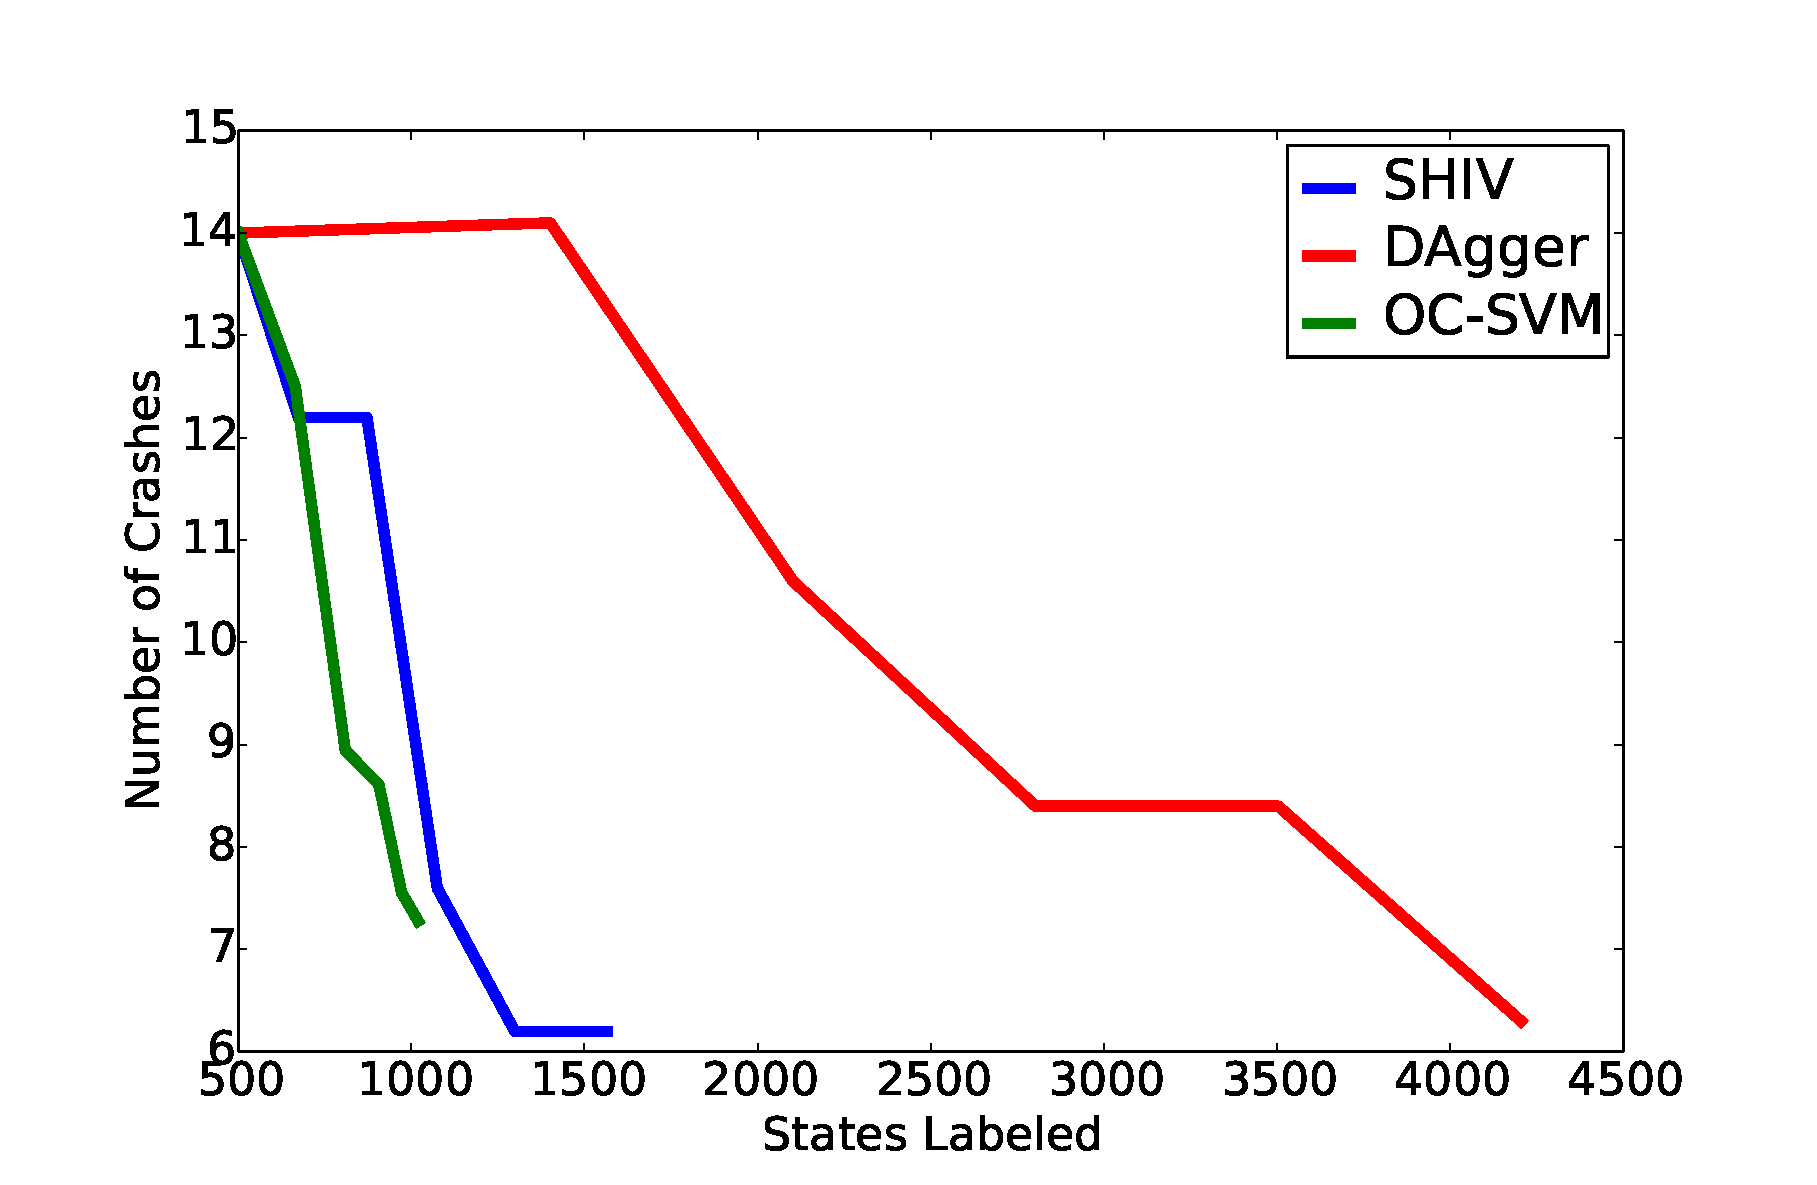
\includegraphics[width=\columnwidth, height=4cm]{figures/dagger_shiv_one_class.eps}
\caption{ \footnotesize We compare normalized performance (i.e. matching the performance of the supervisor) for the Driving Simulator , performance is defined as the number of times the car left the track versus the number of queries made to the supervisor. We plot the performance of DAgger and SHIV, the teal and orange lines. We also plot the performance of our supervisor, who makes non-optimal decisions and has an average performance of 5.4 crashes. Initial results, which are run for 6 iterations each and are averaged over 40 levels, shown in Fig. \ref{fig:car_cost} suggest an $71\%$ reduction in the number of queries needed for SHIV compared to DAgger. Error bars in grey measure the standard error on the mean}
\vspace*{-20pt}
\label{fig:car_cost}
\end{figure}


\subsubsection{Grasping In Clutter in Box2D}

We investigate having a human demonstrator control a simulated robot arm in 2D to reach a target object with out knocking other objects off a table. Grasping an object in a cluttered environment is a common task for a robot in an unstructured environment and has been considered a benchmark for robotic manipulation~ \cite{kitaevphysics,kingnonprehensile}. The task is difficult because modeling the physics of pushing an object is non-trivial and requires knowing the shape, mass distribution and friction coefficient of all objects on the table. We are interested in learning such a policy via human demonstrations. 

We used Box2D a physics simulator to model a virtual world. We simulate a 4 DOF robot arm with three main joints and a parallel jaw gripper as
displayed in Fig. \ref{fig:teaser}(b). SHIV and DAgger do not have access to the underlying dynamics of the simulator and must learn a policy from only demonstrations. 

For input the human demonstrator provides controls through an XBox game controller. The right joystick was used to
    provide horizontal and vertical velocity inputs for the center of the end-effector which were then translated into
robot arm motions by means of a Jacobian transpose controller for the 3 main joint angles. The left `bumper' button on the joystick was used to provide a binary control signal to close the parallel jaw
gripper. The control inputs are hence modeled by the set $\mathcal{U} = \lbrace [-1,1],[-1,1],\lbrace 0,1 \rbrace \rbrace$.  

A state $\bx\in \mathcal{X}$ consisted of the 3 dimensional pose of the six objects on the table (translation and rotation), the 3 joint angles of the arm and a scalar value in the range $[0,1]$ that measured the position of the gripper, $1$ being fully closed and $0$ being opened. For our representation of $\pi_{\theta}$, we used kernelized ridge regression with the radial basis function as the kernel with the default Sci-Kit learn parameters. We defined performance as the sum of the number of objects knocked off the table plus $10$ times the binary value indicating if the object is grasped or not. The order of magnitude difference in cost for grasping the object is to place emphasize on that portion of the task. The bandwidth parameters for SHIV were set to $\sigma_r = 5$ and $\sigma = 6$. For the $\epsilon$ term in the our risk method, we used the median in regression error which was the L2 distance between the predicted control and the true supervisor's control. 

In our experiment, a human demonstrator provided one demonstration and then iterated until the performance was zero during the policy roll out. At each iteration, we sampled the pose of the target object from an isotropic Gaussian with a standard deviation that is  $3\%$ of the width of the table. 

 In Fig. \ref{fig:grasp_cost} , we show the normalized performance averaged over 8 rounds for SHIV and DAgger. Supporting our hypothesis, our results suggests that SHIV can achieve the same performance with a 64\% reduction in the number of examples needed.

\begin{figure}[t!]
\centering
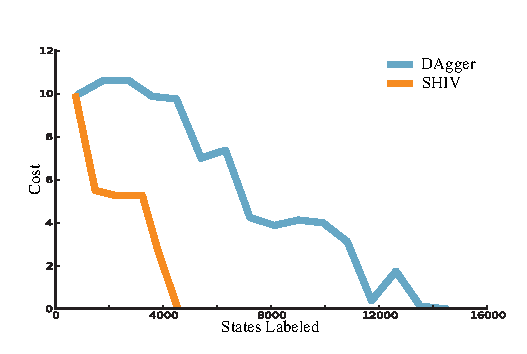
\includegraphics[width=\columnwidth, height=4cm]{figures/grasp_clutter.eps}
\caption{ \footnotesize We compare normalize performance (i.e. mathcing the performance of the supervisor) for Grasping in Clutter domain, performance is defined as the sum of the number of objects knocked off the table plus 10 times the binary value indicating if the object is grasped or not. Initial results, which are averaged over 8 different trials suggest a $64\%$ reduction in the number of queries needed for SHIV compared to DAgger,}
\vspace*{-20pt}
\label{fig:grasp_cost}
\end{figure}




\subsubsection{Surgical Needle Insertion}

Robotic Surgical Assistants (RSAs) are frequently used for procedures such as: prostectomy, uterectomy, and tumorectomies within the abdominal and thoracic cavities with high success rates~\cite{van2013laparoscopic,darzi2004impact}. Introducing autonomy of surgical sub-tasks has the potential to reduce cognitive load and facilitate supervised autonomy for remote tele-surgerical procedures.

Suture tying in surgery is a manually intensive task that can occur frequently through out a surgery. One important step
in suture tying is properly placing a needle in an initial configuration for insertion. Misplacement of this the needle
can lead to suture failure and potentially rupture the surrounding tissue \cite{liu2015optimal}. In this experiment, we
are interested in learning to correct bad initial poses to the proper pose as shown in Fig.
\ref{fig:support_example}. Dr. Douglas Boyd, a surgeon and professor at UC Davis, provided us with a collection of demonstrations on a Intuitive Surgical Da Vinci Research Kit \cite{AnnualReport2014}.

Dr. Boyd demonstrated a set of trajectories that each started at an initial attempted needle insertion pose $P_0$ and
applied the necessary corrections to achieve a goal pose $P_G$. The time horizon, $T$ of each trajectory was on average 80.  We used three of these demonstrations as our initial
dataset $\mathcal{D}_0$, thus $|\mathcal{D}_0| = 240$. In order to study convergence of both SHIV and DAgger, we chose to create a synthetic expert for online learning part. The expert controller computed the transformation between the desired insertion pose and the current pose  by calculating the inverse of a transformation matrix, $C = P_0P_G^{-1}$. Then converted $C$ to the associated lie algebra vector $c \in \mathbb{R}^6$ for $SE(3)$ and normalize it to the average magnitude of the control,  $||\bar{c}_D||$, Dr. Boyd applied. 

The policy $\pi_{\theta}$ was represented as kernel ridge regression with the default values given in Sci-Kit learn. The state $\mathcal{X}$ was  a 16 dimensional vector consisting of the elements in the pose $P$ vector. The control space $\mathcal{U}$ was a $\mathbb{R}^6$ vector representing the Lie algebra. 

For the $\epsilon$ term in the our risk method, we used the median in regression error which was the L2 distance between the predicted control and the true supervisor's control. 
regions respectively. The bandwidth, $\sigma$, in the rbf kernel was set to $2$ and $\sigma_b = 1$.

For trials we sample a start position from a Gaussian on the translational component of $P_0$ with isotropic variance of
$0.1$ cm. The distance between initial $P_0$ and $P_G$ is roughly $3$ cm. Performance is measured in
terms of Euclidean distance in translational component, which is in centimeters. We run DAgger and SHIV both for 20 iterations and average over 40 different starting positions.

 In Fig. \ref{fig:grasp_cost} , we show the normalized performance (i.e. 1 corresponds to matching the supervisor) averaged over 40 rounds for SHIV and DAgger. Supporting our hypothesis, our results suggests that SHIV can achieve the same performance with a $67\%$ reduction in the number of examples needed.


\begin{figure}[t!]
\centering
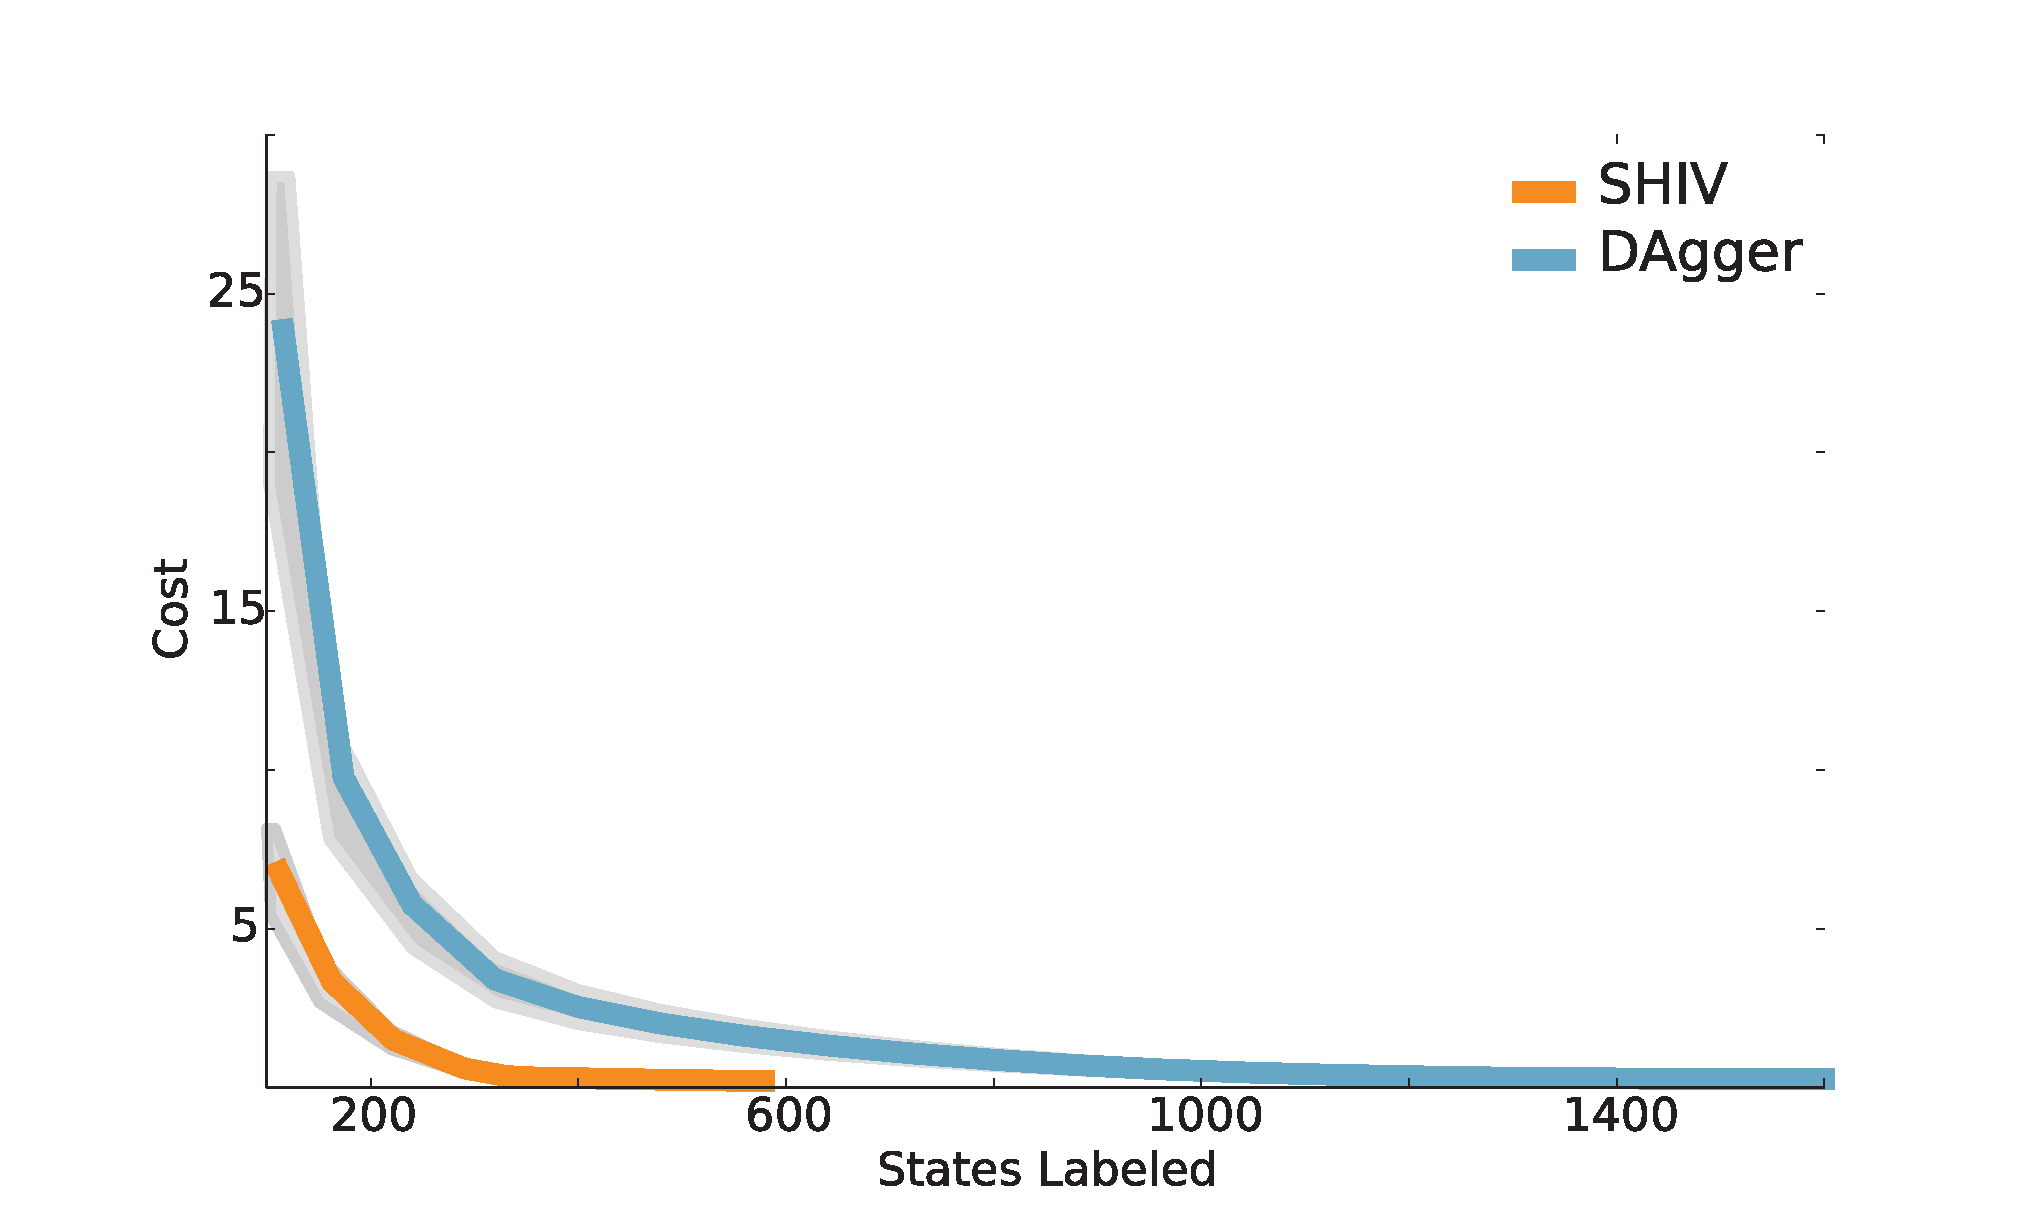
\includegraphics[width=\columnwidth, height=4cm]{figures/needle_insertion_results.eps}
\caption{ \footnotesize We compare normalized performance (i.e. matching the performance of the supervisor), performance is defined as the euclidean distance between translation in centimeters. In Fig. \ref{fig:car_cost}, we plot the performance of DAgger and SHIV.  Initial results, which are run for 20 iterations each and are averaged over 40 different initial starting positions, shown in Fig. \ref{fig:car_cost} suggest an $67\%$ reduction in the number of queries needed for SHIV compared to DAgger. Error bars in grey measure the standard error on the mean}
\vspace*{-20pt}
\label{fig:needle}
\end{figure}


\subsection{SHIV Analysis}\label{sec:car}



\subsubsection{Comparison to active learning approaches.}

 We compare five active learning methods. We compare our combined notion of risk (Fig. \ref{fig:support_example}(d)), with risk based on novelty alone (Fig. \ref{fig:support_example}(c)) in order to test whether carving out regions that have been misclassified previously is valuable. 

We also compare against two baselines typically used in active learning. The first is confidence based on distance from the classification hyperplane \cite{tong2002support} (Fig. \ref{fig:support_example}(a)). We set the threshold distance to the average distance from the hyperplane for the mis-classified points in $\mathcal{D}_0$, which consisted of two demonstrations from our solver. 

The second baseline is Query By Committee (Fig. \ref{fig:support_example}(d)), which has a committee of different hypothesis estimators and points are marked risky if the committee disagrees. Our committee which was trained via bagging~\cite{breiman1996bagging}.  To obtain a committee, we divided the training data into 3 overlapping subsets, each with 80\% of the data. We trained a Linear SVM on each subset. If the three classifiers agreed with each other the point was determined low risk and if they disagree it was determined high risk. 
%We finally compared our combined risk approach against the traditional One Class SVM without the "carving out". 

We compare against another novelty detection method as well called Maximal Mean Discrepancy (MMD), which evaluates how close a point is to the distribution using kernel density estimate and adds the variance of the distribution in the dataset $\mathcal{D}$~\cite{kim2013maximum}.  We set bandwidth of the kernel as the same as our modified One Class SVM and the $\alpha$ decision boundary is set by sorting the MMD value of the states and picking an $\alpha$ such that the lowest $10\%$ are marked as risky. This is in similar spirit to $\nu = 0.1$. 

We run each query selection method over 50 different car tracks in the driving simulator domain. We measured the percentage of truly risky states, encountered during the first policy roll out, that  are estimated to be safe by the active learning technique. The active learning techniques are trained on the initial demonstrations $\mathcal{D}_0$, which is different then the distribution being sampled from, $p(\bx|\theta_0)$, in this experiment.

 Fig. \ref{fig:active_comp}  plots the performance for each query selection method, averaged over 50 tracks. We observe a significant performance improvement with methods based on classification based novelty detection compared to confidence,query by committee and MMD. Furthermore, using the combined measure of risk performs better than relying solely on the One Class SVM. 

\subsubsection{Sensitivity Analysis to Risk Sensitivity Parameter}

 To analyze the sensitivity of our method we varied the risk sensitivity  parameter or $\sigma$ of the decision function $g_{\sigma}$, or Eq. $\ref{eq:decision_func}$. $\sigma$ is a measure of how much risk we allow, with smaller $\sigma$s leading to more risk-adverse behavior. SHIV was ran for 6 iterations and averaged over 40 different randomized polygonal tracks. 

 For each  $\sigma$, we measure the final cost performance of the policy $\pi_{\theta}$ after 6 iterations and the number of examples SHIV requested from the supervisor. 

 As shown in Table \ref{tab:sens}, small $\sigma$, $\sigma = 1$, corresponds to always asking for help (many states labeled) and very large sigma, $\sigma = 350$, relates to  less data being used, but worse performance. However, $\sigma$ values between $150$ and $250$ all achieve similarly good performance, suggesting that SHIV is robust to the choice of a particular $\sigma$.


\begin{table}[t]
\centering
\begin{tabular}{ R{2.5cm}||R{1.65cm}|R{1.65cm} }
 %\hline
 %\multicolumn{4}{|c|}{Sensitivity Analysis for Convergence to Best Grasp for Thompson sampling} \\
 %\hline 
 \hline
\specialcell{\bf Risk  Sensitivity ($\sigma$)} & \specialcell{\bf Performance} & \specialcell{\bf States  Labeled} \\
 \hline
 1 & 5.8 & 4122 \\
 50 & 5.7&  3864 \\
 150& 5.9 &  1859 \\
200 & 6.1 & 1524 \\
250 & 6.3 & 1536 \\
350 & 13.2 & 521\\

 %\hline
\end{tabular}
   \caption { \footnotesize  An analysis of the sensitivity risk sensitivity parameter,$\sigma$, of Eq. \ref{eq:decision_func}, or the decision function for risky or safe. SHIV was run for 6 iterations and averaged over 40 different randomized polygonal tracks. Small $\sigma$, $\sigma = 1$, corresponds to always asking for help and very large sigma, $\sigma = 350$, relates to a lot less data being used, but decreased performance. 
   }
		\tablabel{opt-p-comparison}
		\label{tab:sens}
\vspace*{-10pt}
\end{table}


\begin{figure}[t]
\centering
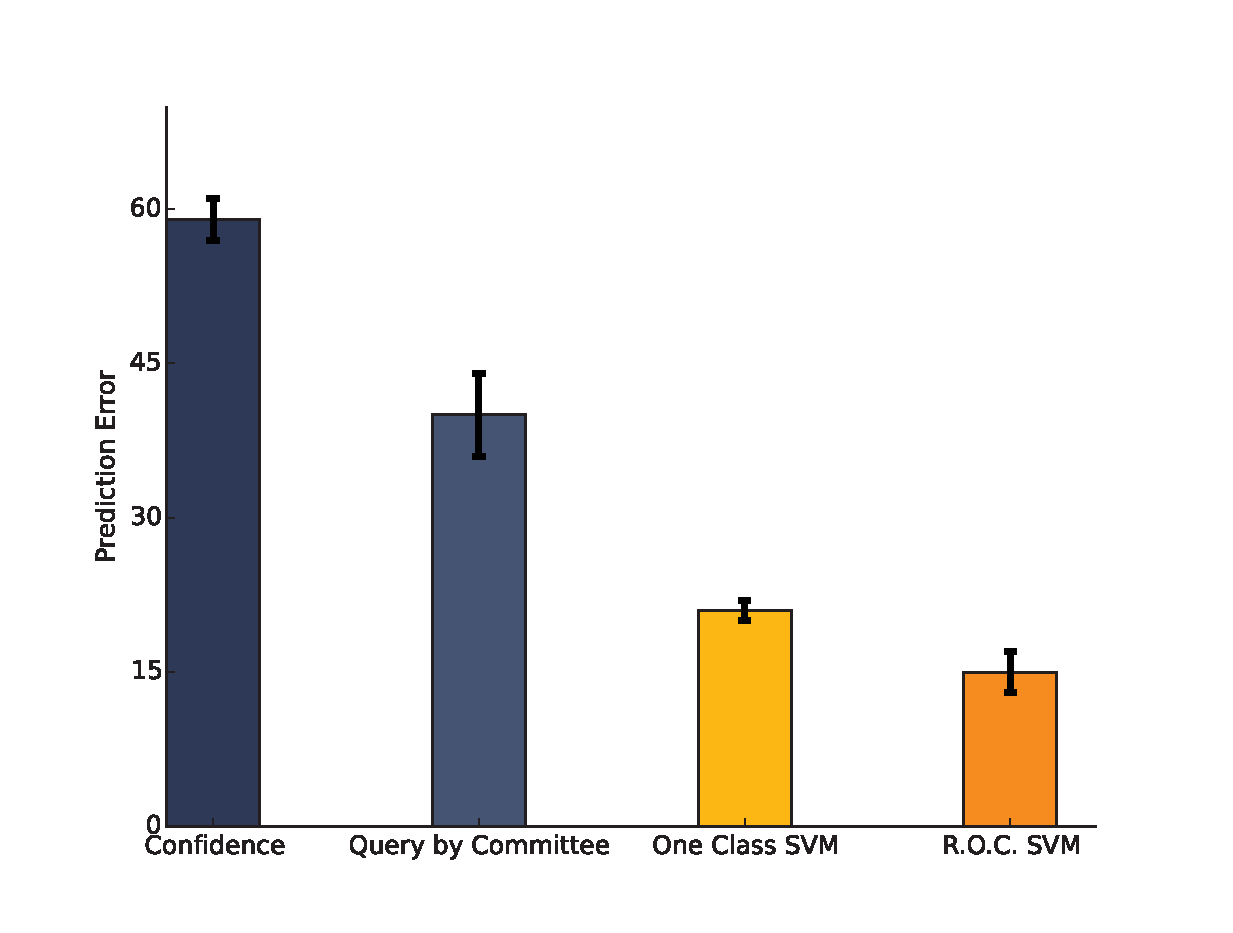
\includegraphics[width=\columnwidth, height=4cm]{figures/risk_bar.eps}
\caption {  \footnotesize A comparison of different active learning approaches in terms of the percentage of risky states that are estimated to be safe by the active learning technique during the first policy roll out. We compare against a confidence estimate of distance to hyperplane,Maximal Mean Discrepancy, query by committee for 3 hypothesis classifiers, the One Class SVM, and our modified One Class SVM, marked as SHIV.  Results  are averaged over 50 tracks and the policy $\pi_\theta$ is represented as a Linear SVM. Error bars measure the standard error on the mean.
   }
\vspace*{-20pt}
\label{fig:active_comp}
\end{figure}





\section{Discussions and Future Work}
Online LfD has been successful on an array of tasks~\cite{NIPS2014_5421,ross2010reduction}, however it can place significant burden on a supervisor. Our algorithm, SHIV, implements stream-based active learning with a query selection method that evaluates risk in a manner tailored to non-stationary and high-dimensional state distributions. We empirically evaluated our method on three different domains: a driving simulator, grasping in clutter and surgical needle insertion. Results suggests up to a $70\%$ reduction in the number of queries to the supervisor. 

SHIV has several limitations. For instance, the selection of the value of $\sigma$ can affect performance and a poor choice could result in the algorithm becoming offline imitation learning, as shown in Table \ref{tab:sens}. Future work will look at better understanding the relationship of $\sigma$ to the function $\pi_{\theta}$ and how to automatically select it. 

Furthermore, to update the decision function $g_{\sigma}$ requires solving a quadratic program, which has an upper bound computationally complexity of $O(n^3)$ in the number of data points. This can effect the ability of using our modified One Class SVM for larger problems. While, Scholk{\"o}pf et al. provides an efficient optimization that empirically scale quadratically \cite{scholkopf2001estimating} for very large datasets this can still be burdensome. Future work will look at using techniques such as random features or PCA on the kernel Gram matrix to allow for better scaling \cite{scholkopf2002learning}.
  
 




\bibliographystyle{IEEEtranS}
\bibliography{references}



\end{document}
